\documentclass{beamer}
\usepackage{etex}
\usepackage[utf8]{inputenc}

\usepackage{amsmath}
\usepackage{amsfonts}
\usepackage{amssymb}
\usepackage{amsthm}
\usepackage[ukrainian,russian]{babel}

\usepackage{fontenc}
\usepackage{graphicx}
\usepackage{wrapfig}
\usepackage{tikz}

\usepackage{ulem}

\usepackage{listings}
\usepackage{color}
\usepackage{hyperref}
% \usepackage[unicode,pdfusetitle, bookmarks=true, bookmarksnumbered=true,bookmarksopen=true,bookmarksopenlevel=1]{hyperref}
% \hypersetup{backref,colorlinks=true,linkcolor=blue,citecolor=green,bookmarks=false}
\usepackage{latexsym,url}
%  \bra and \ket are already defined in Qcircuit
% \usepackage{braket} 
\usepackage{multirow}



\usetheme{Warsaw}
\defbeamertemplate*{footline}{shadow theme}
{%
  \leavevmode%
  \hbox{\begin{beamercolorbox}[wd=.5\paperwidth,ht=2.5ex,dp=1.125ex,leftskip=.3cm plus1fil,rightskip=.3cm]{author in head/foot}%
    \usebeamerfont{author in head/foot}\insertframenumber\,/\,\inserttotalframenumber\hfill\insertshortauthor
  \end{beamercolorbox}%
  \begin{beamercolorbox}[wd=.5\paperwidth,ht=2.5ex,dp=1.125ex,leftskip=.3cm,rightskip=.3cm plus1fil]{title in head/foot}%
    \usebeamerfont{title in head/foot}\insertshorttitle%
  \end{beamercolorbox}}%
  \vskip0pt%
}


\author{Ширай Андрей}
 \institute{Department of Nanotimberlogy,\\Miskatonic University}
\title{Fundamental Limitation on Applicability of Statistical Methods to Study of Living Organisms and Other Complex Systems}
\date{\today}

\newtheorem{defin}{Определение}
\newtheorem{theor}{Теорема}
\newtheorem{astat}{}
\newtheorem{stat}{Постулат}



\begin{document}
\frame{\titlepage}

\frame{
\frametitle{О чем речь?}
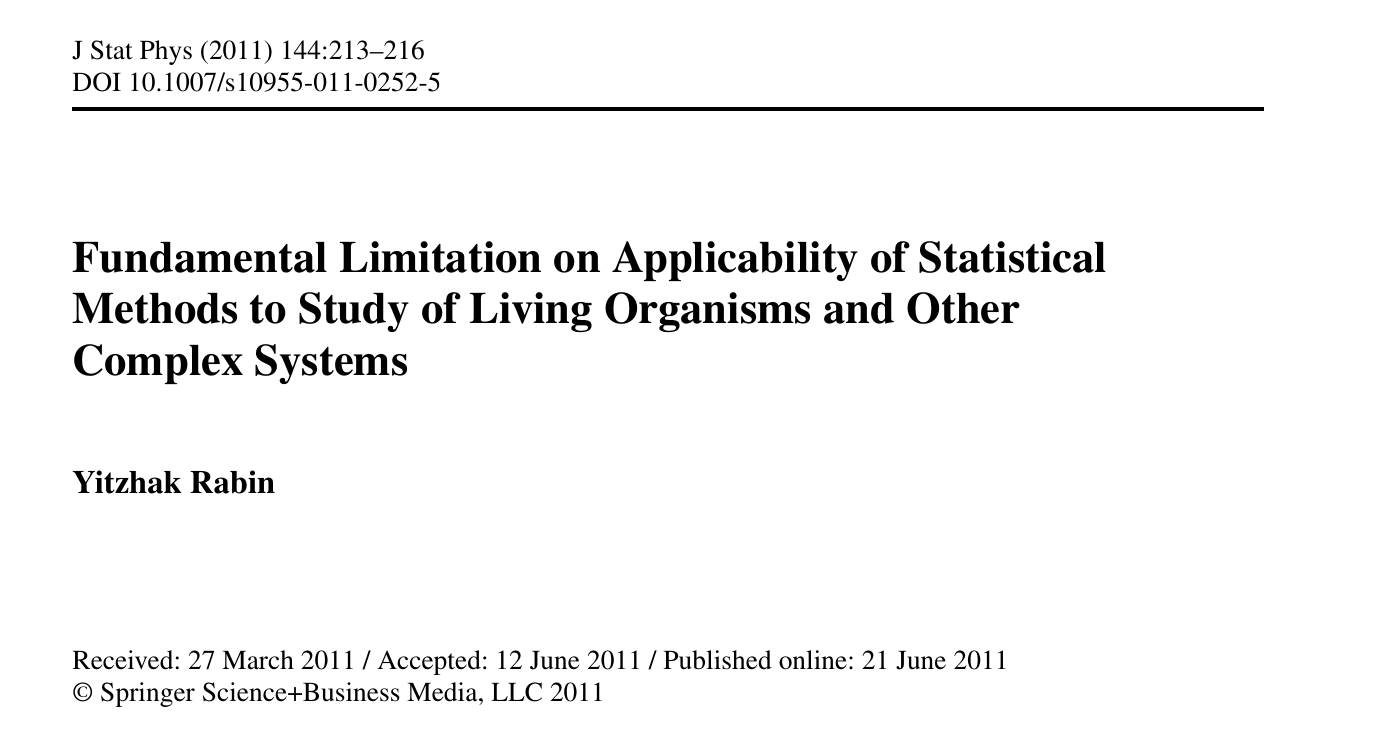
\includegraphics[scale=0.35]{1}
}
\frame{
\frametitle{Lies, damned lies, and \textbf{statistics}}
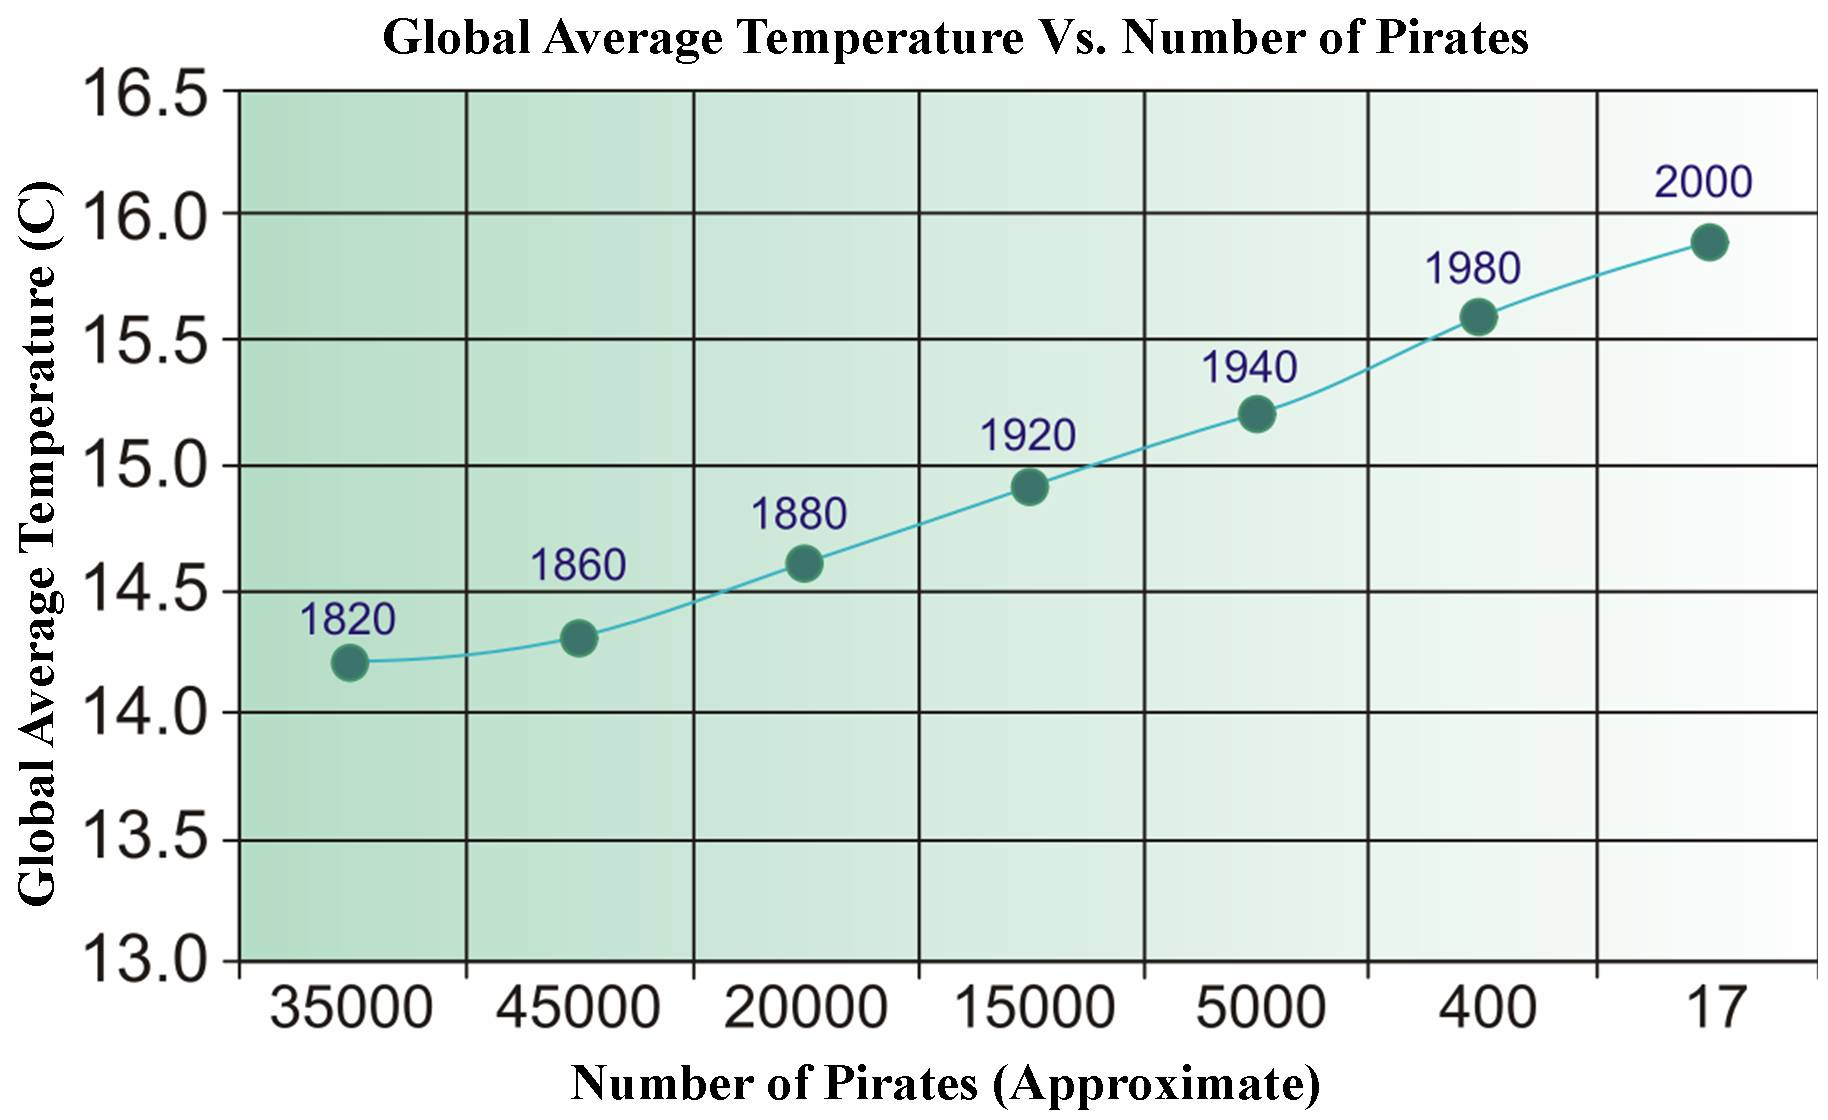
\includegraphics[scale=0.35]{pirates}
}

\frame{
\frametitle{The Dreams in the Witch House}
\begin{itemize}
 \item Предположим у нас есть $ N \gg 1 $ ``идентичных'' систем с каким-то свойством $M$(Которое принимает большое количество возможных значений $M_x \gg 1$)
 \item $N \gg M_x$
 \item По результатам измерений мы получем гистограмму $P(x_i)$
 \item В простейшем случае(если $P(x_i=a)\simeq1$) мы получим $P(x)=A e ^{-\frac{(x-a)^2}{2\sigma^2}}$, проводим оценку $\sigma$
\end{itemize}

}

\frame{
\frametitle{The Horror at Red Hook}
\begin{itemize}
 \item $N$, которое $ N \gg 1 $ хороше, если будет равно 50
 \item ... и которые не идентичны.
 \item Мы не знаем как мерять $M$
 \item ... поэтому $M_x =2$
 \item Система не будет определяться свойством X\footnote{Закон подлости}
\end{itemize}

}

\frame{
\frametitle{The Horror at Red Hook}
\begin{itemize}
 \item $N$, которое $ N \gg 1 $ хороше, если будет равно 50
 \item ... и которые не идентичны.
 \item Мы не знаем как мерять $M$
 \item ... поэтому $M_x =2$
 \item Система не будет определяться свойством X\footnote{Закон подлости}
\end{itemize}
\[
 \operatorname{P}(x)=\operatorname{P}(x\mid y) = A e ^{-\frac{(x-\operatorname{a}(y))^2}{2\operatorname{\sigma}(y)^2}}
\]


}


\frame{
\frametitle{Ex Oblivione}
\begin{itemize}
 \item Почему эта проблема не затронула физику?
\end{itemize}

}
\frame{
\frametitle{Ex Oblivione}
\begin{itemize}
 \item Почему эта проблема не затронула физику?
 \item Законы сохранения!
\end{itemize}

}
% \frame{
% \frametitle{We have a plan!}
% 
% \begin{itemize}
%  \item Исторический экскурс.
%  \item Как это работает.
%  \item Примеры физических реализаций.
%  \item Квантовые алгоритмы Шора(факторизация) и Гровера(поиск по неупорядоченной БД).
%  \item Как это повлияет на надежность криптосистем?
%  \item Как квантовая информатика повлияла на другие направления теоретической 
% информатики/математики/физики.
%  \item Моделирование квантовых вычислений
% \end{itemize}
% 
% }

% % % % % % % % % % % % % % 


% % % % % % % % % % % % % % 

\frame{
 \frametitle{Feci, quod potui, faciant meliora potentes}
\begin{center}
\Huge Dixi\end{center}
}



%%%%%%%%%%%%%%%%%%%%%%%%%%%%%%%%%%%%%%%%%%%%%%%%%%%

% \frame{
% \frametitle{}
% 
% \begin{figure}[ht]
%  \includemovie[
%  poster,
%  text={\small P vs NP}
% ]{0.5\linewidth}{0.5\linewidth}{pnp.mp4}
% \end{figure}
% }

\end{document}
